\section{Exploration Environment}
\label{sec:app}

Consider adding this section to describe the Regulus/IPyRegulus system.

Designed to facilitate an \textit{Analysis First} approach. Enable analysts to visualize data as part of their analysis workflow and employ their functions as models, measures and filters. 

\begin{figure}
    \centering
    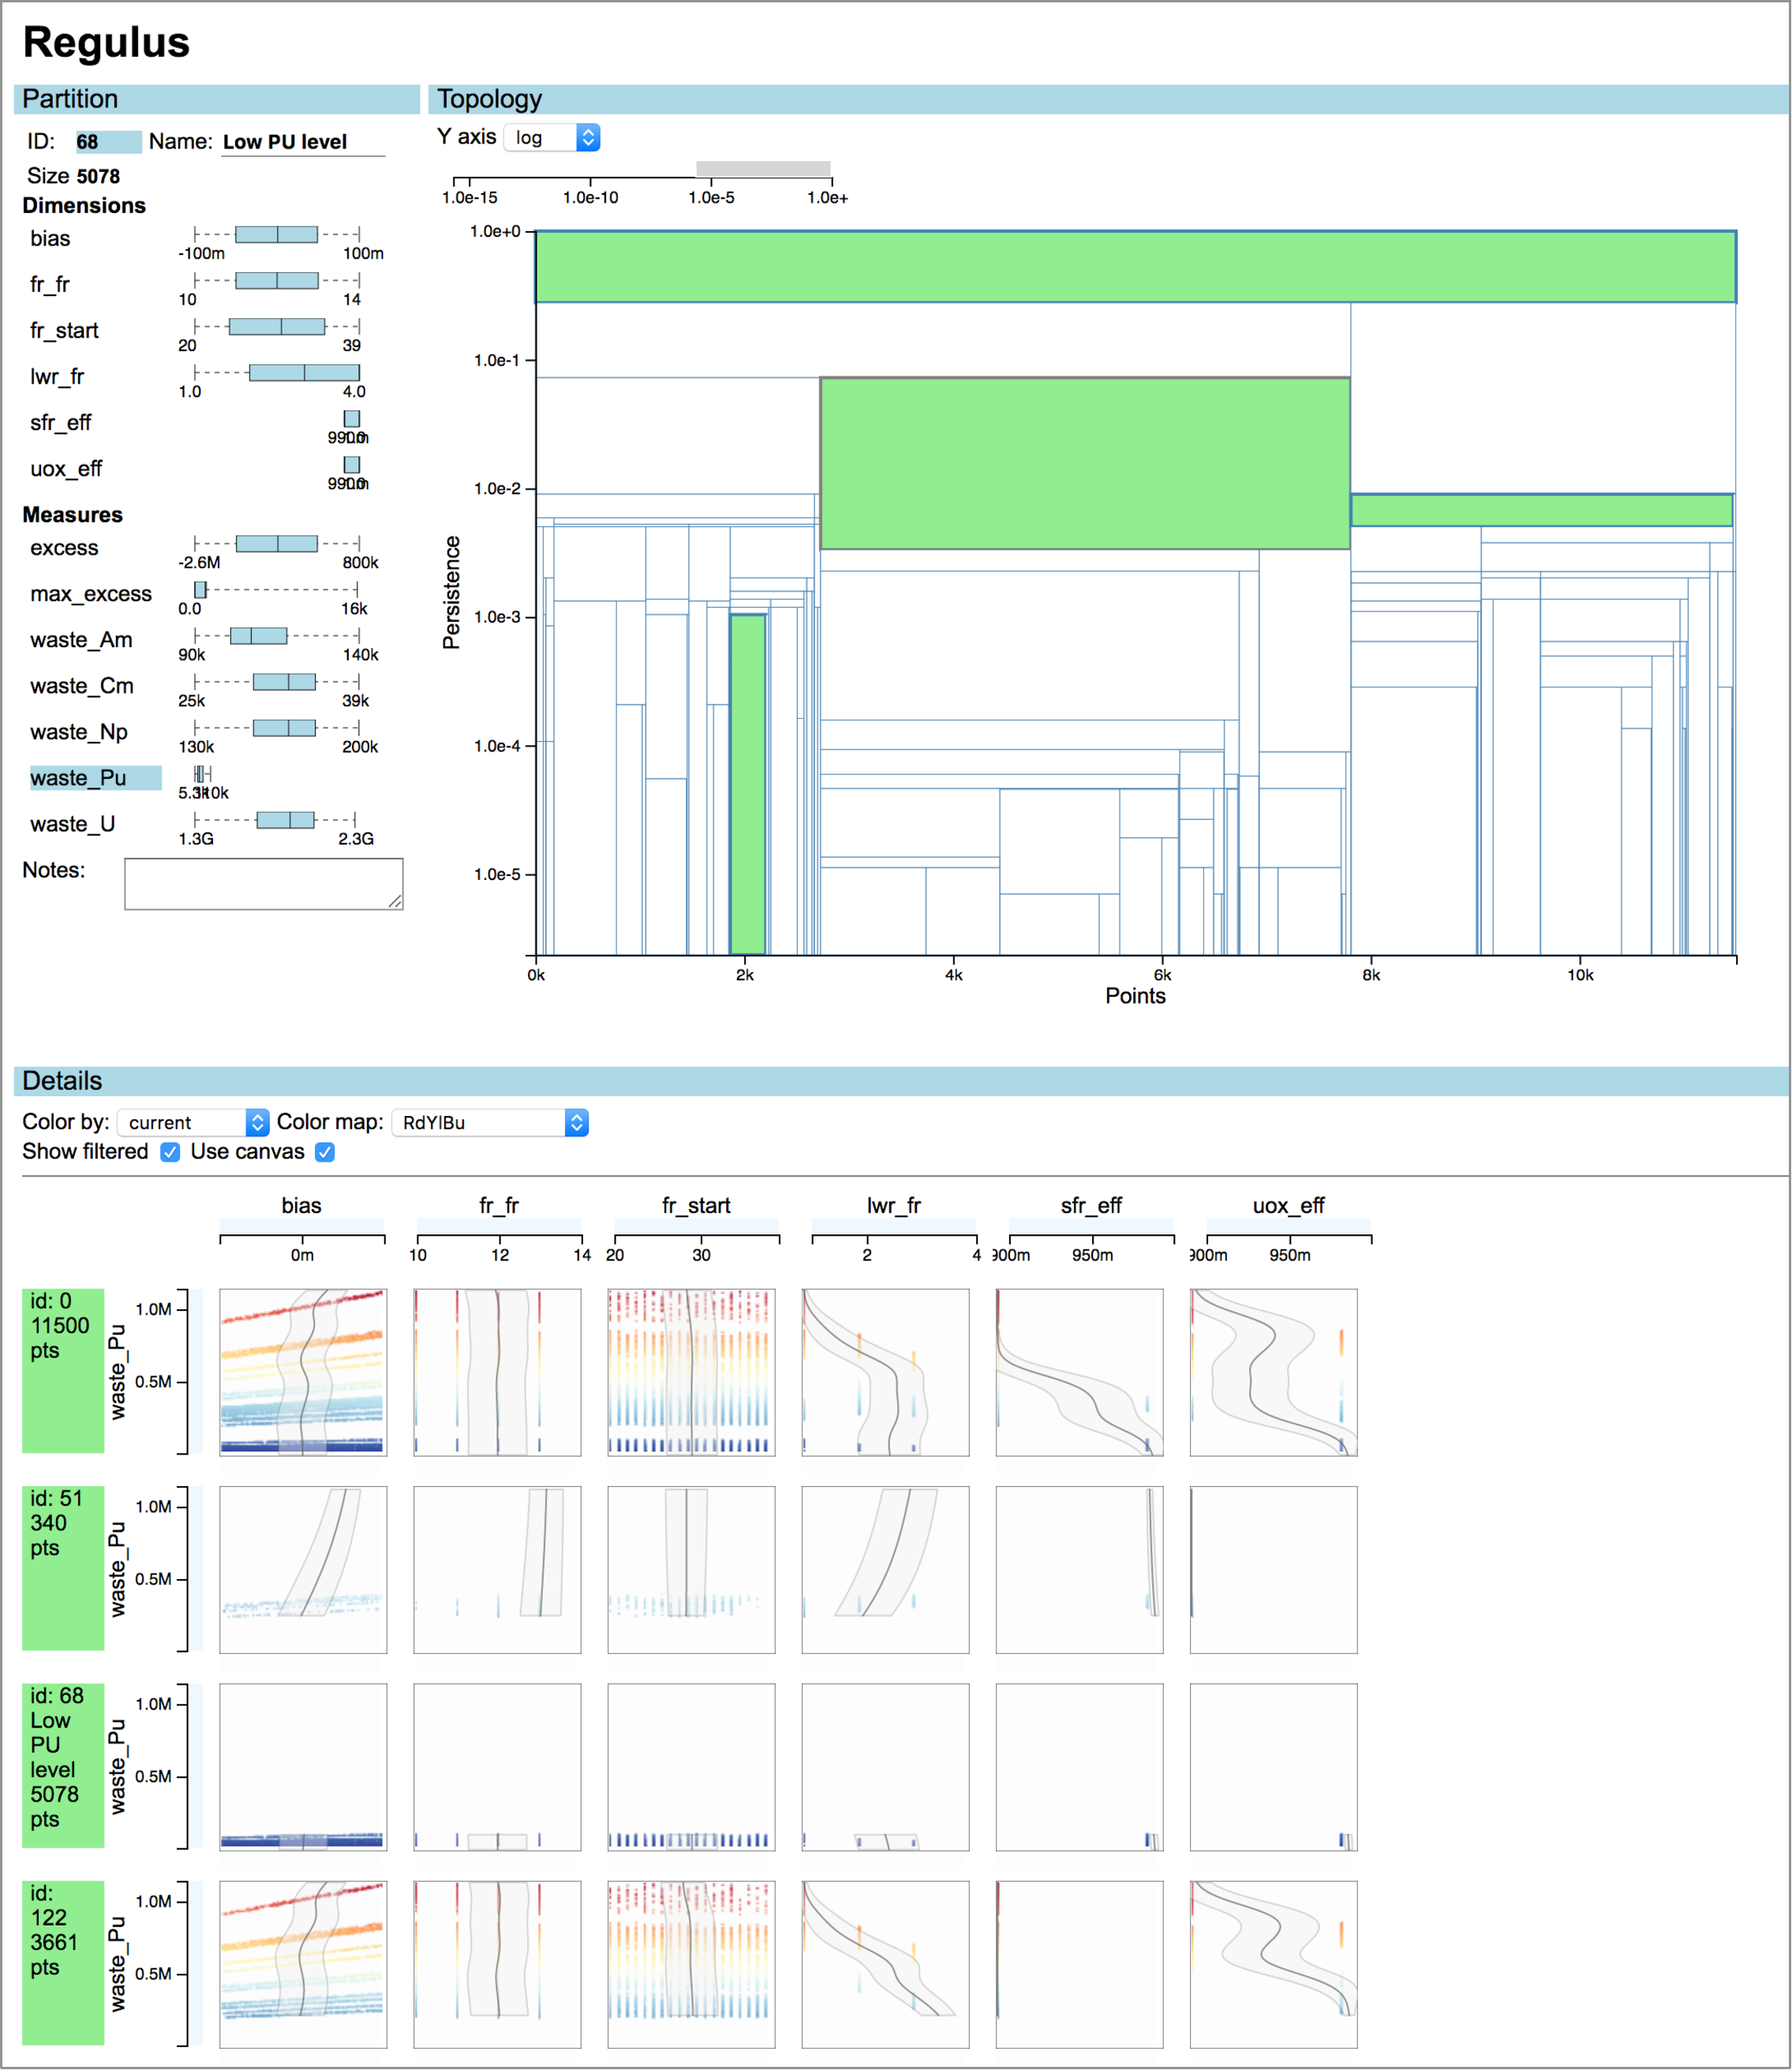
\includegraphics[width=\linewidth]{regulus-js}
    \caption{Visualization first implementation}
    \label{fig:regulus-js}
\end{figure}

Software consist of \textbf{Regulus}: a pure python package and \textbf{IPyRegulus}: interactive widgets for JupyterLab. 

\subsection{Regulus Attributes}
\label{sec:attr-impl}

\subsubsection{Caching}
\label{sec:caching}
Our aim is to avoid computing attributes, such as models and measures, for all the nodes. Instead, each attribute is associate with a generator function and a cache. An attribute value for a node will be computed using the generator function the first time it is requested and the value will be stored in the cache. If the user saves a Regulus object to a file, the generator function and the cached values will be saved in the file and will be loaded with the Regulus object the next time.

\begin{lstlisting}[language=Python, caption=Attributes can be used to reduce computations., float=htb, label='fig:model-fitness]
from sklearn import linear_model as lm

def linear_model(tree, node):
    model = lm.LinearRegresssion()
    model.fit(node.data.x, node.data.y)
    return model
    
def fitness(tree, node):
    model = tree['linear_model'][node]
    return model.score(node.data.x, node.data.y)
 
# Naive implementation 
# Not suitable for derived trees
# See Chained Attributes section
def parent_fitness(tree, node):
    parent_model = tree['linear_model'][node.parent]
    return parent_model.score(node.data.x, 
                              node.data.y)
    
tree.add_attr(linear_model)
tree.add_attr(fitness)
tree.add_attr(parent_fitness)
\end{lstlisting}

\subsection{Chained Attributes}
\label{sec:chained_attrs}

A Regulus tree may be derived from another, such as when one tree is a simplification of another (see \autoref{sec:simplification}). We want to avoid computing attributes for the derived tree that were already implemented in the original tree such a node fitness. However, some attributes depends on the tree structure.  

\begin{lstlisting}[language=Python, 
    caption=Chained attributes. Parent/child relation depends on the current tree structure, float=htb, label=fig:relative-fitness]

def relative_fitness(tree, has_model, has_pts):
    return tree['linear'][has_model].score(has_pts.data.x, has_pts.data.y)
    
def parent_fitness(tree, node):
    return tree['relative_fitness'][node.parent, node]

def child_fitness(tree, node):
    return tree['relative_fitness'][node, node.parent]    
\end{lstlisting}

\subsection{IPyRegulus}
\label{sec:ipyregulus}

A set of visualization widgets in a jupyter notebook and in particular in JupyterLab.

Discuss the benefits of using a notebook:
\begin{itemize}
    \item linear order
    \item repeatably
    \item scripted
\end{itemize}

A single model can be viewed several times. 

We want to avoid moving the data (points) and the Regulus structure (partitions) for each view. 

\begin{description}
\item[DataWidget] represents a model of the data and all the Morse-Smale partitions 
\item[DetailsView] refers to a DataWidget for points
\item[TreeWidget] represents a Regulus Tree and a set of attributes that were requested for visualization. Has not data points. A model with no visualization
\item[TreeView] refers to a TreeWidget for the tree structure.
\end{description}

\subsubsection{Side Panel}
\label{sec:sidepanel}
The need for a side panel that can be controlled by the user (add, resize, collapse views).

\subsubsection{Coordinated Multiple Views}
\label{sec:cmv}

See \autoref{fig:cmv}.

\begin{figure}[htb]
    \begin{center}
     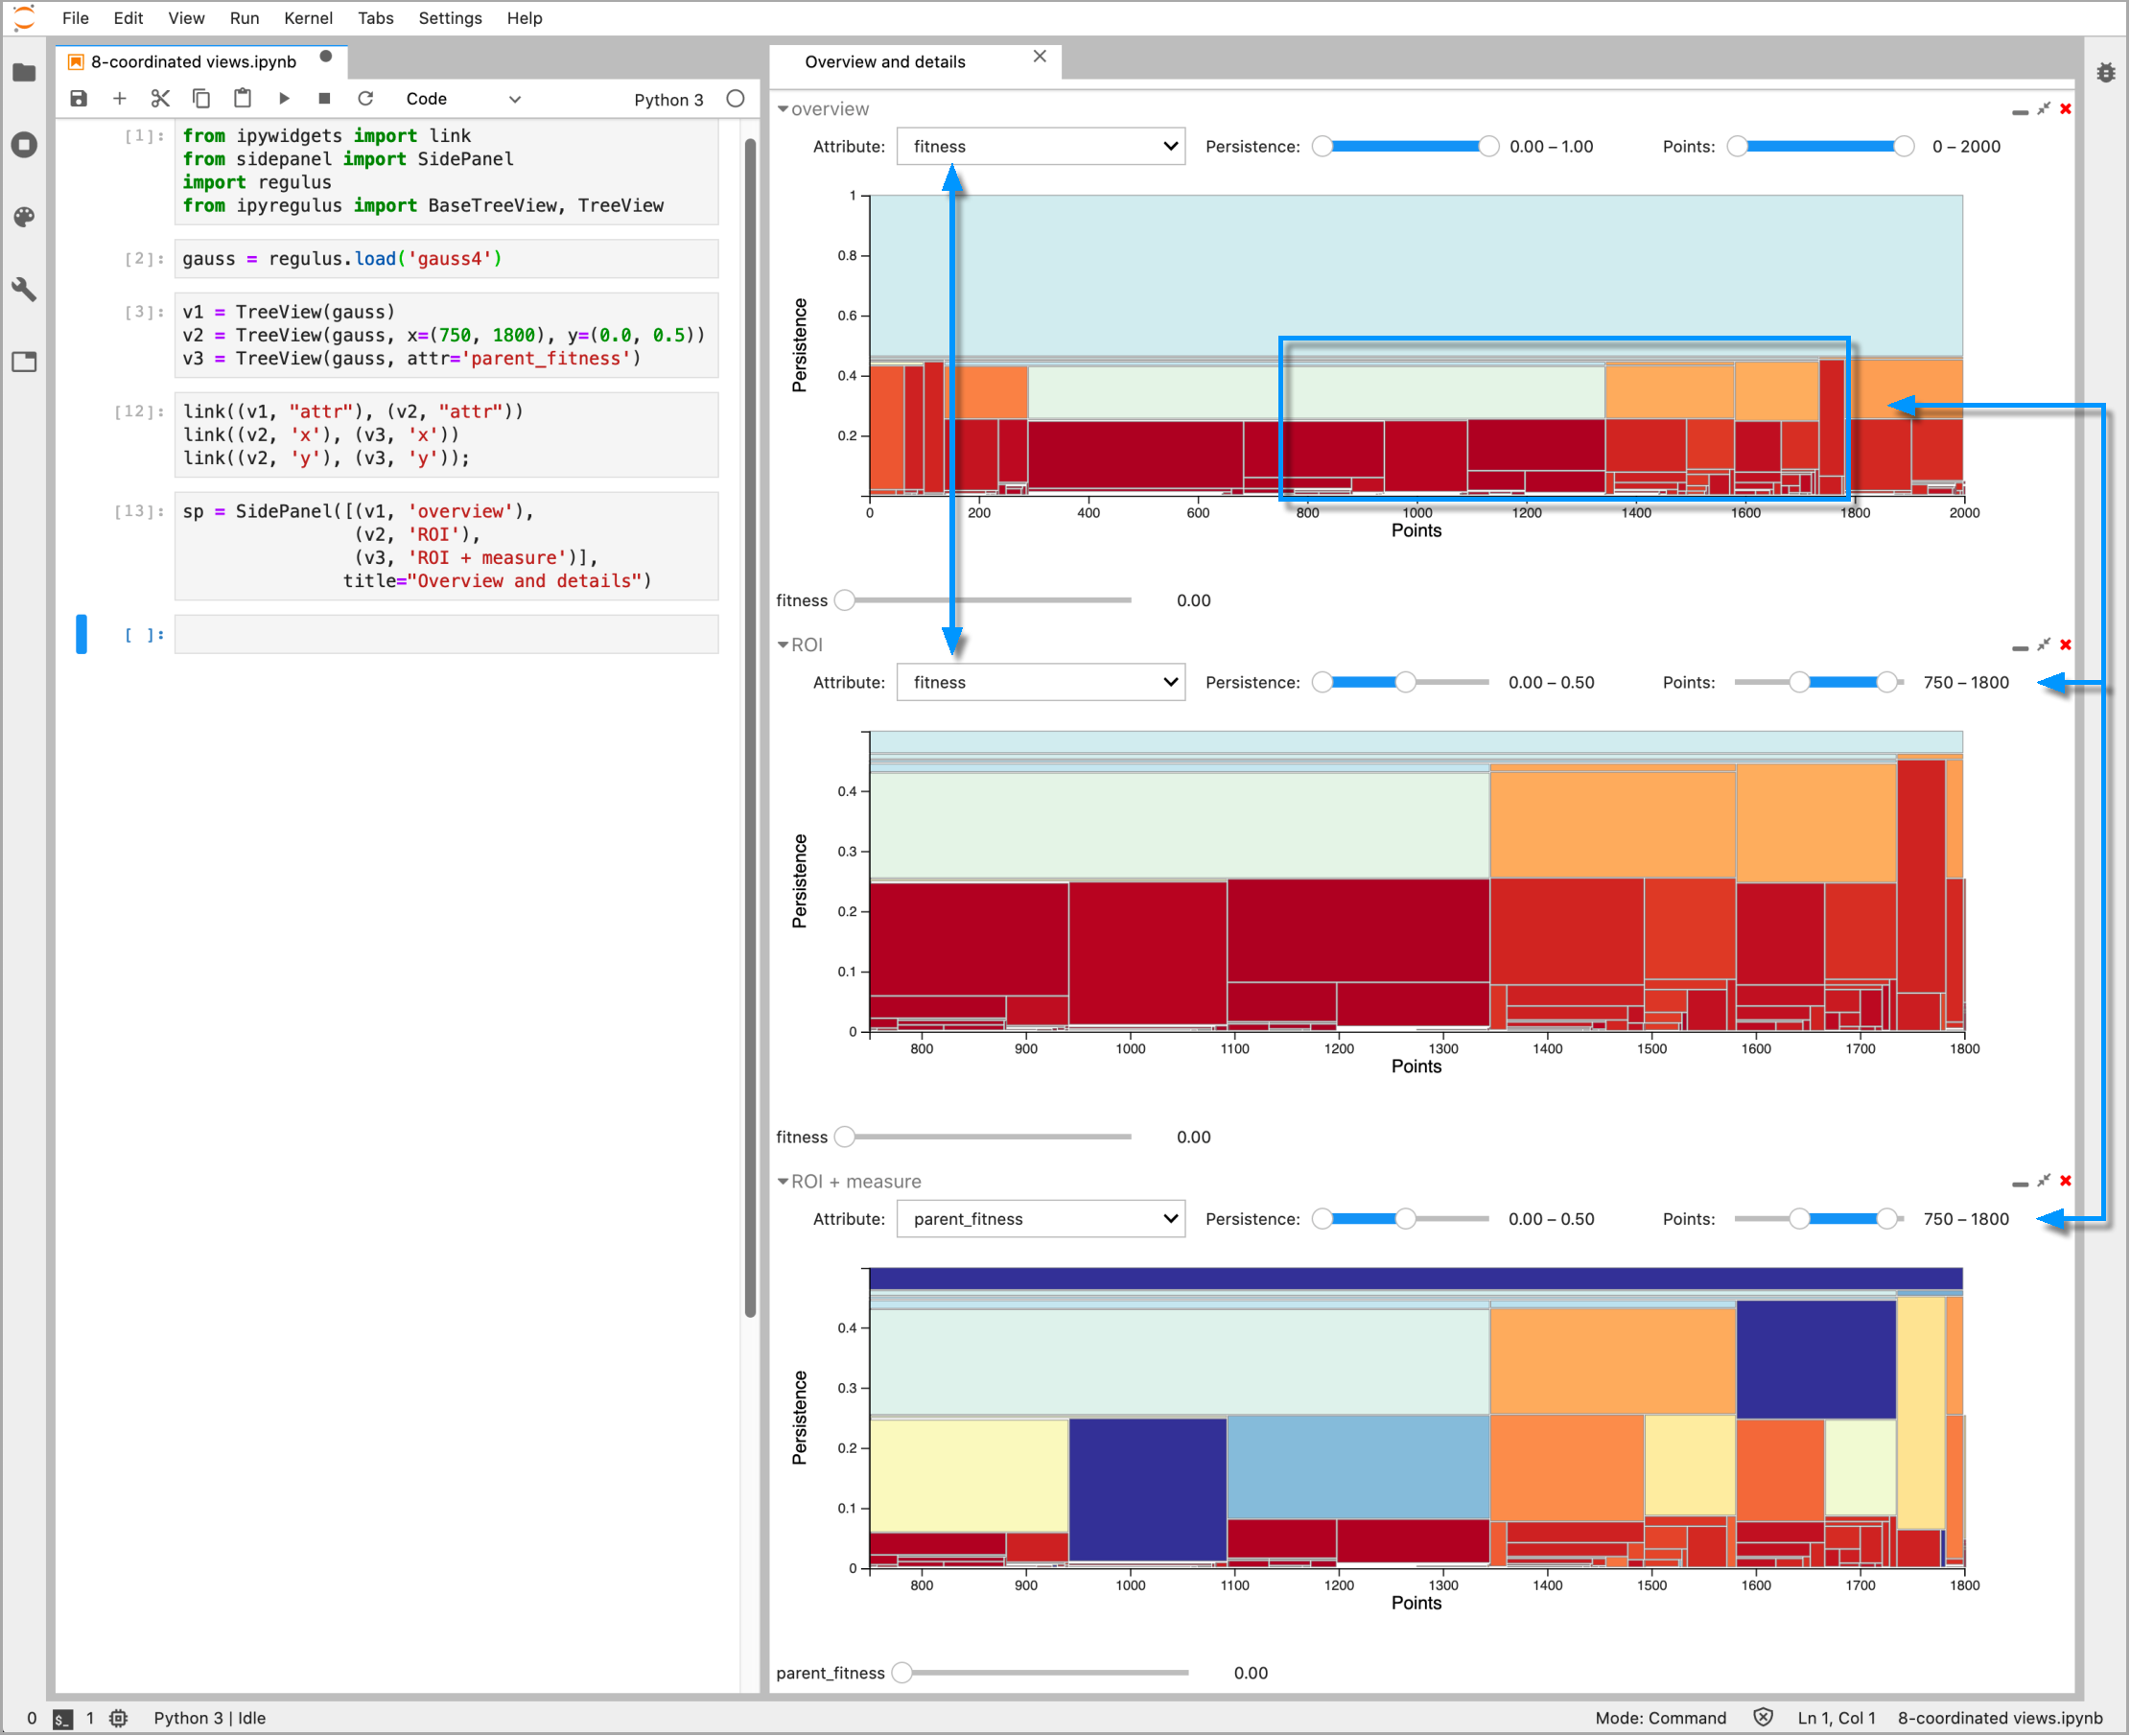
\includegraphics[width=\linewidth]{cmv}
    \caption{On the fly views coordination. Three views of the same tree in a SidePanel. Top and and middle views shows the same attribute (fitness) while the middle and bottom show the same region of interest. Changing the ROI in the middle or bottom views will update the other view.} 
    \label{fig:cmv}
    \end{center}
\end{figure}

\subsubsection{Tree Dependency}
\label{sec:tree-dependency}

Instead of explicit dataflow model with modules and ports.
